% LuaLaTeX; the supplied uetgraduation.cls is not modified.
\PassOptionsToPackage{no-math}{fontspec}
\RequirePackage{fix-cm}
% Keep the supplied UET class unchanged. Replace only unavailable font names.
% Liberation Serif is a freely licensed, metric-compatible Times alternative.
\newif\ifReportFontFallback
\AddToHook{package/fontspec/after}{%
  \IfFontExistsTF{Times New Roman}{}{%
    \global\ReportFontFallbacktrue
    \NewCommandCopy\ReportOriginalSetMainFont\setmainfont
    \RenewDocumentCommand\setmainfont{O{} m O{}}{%
      \IfFontExistsTF{#2}{%
        \ReportOriginalSetMainFont[#1]{#2}[#3]%
      }{%
        \ReportOriginalSetMainFont[#1]{Liberation Serif}[#3]%
      }%
    }%
  }%
}
\AddToHook{package/mathfont/after}{%
  \ifReportFontFallback
    \NewCommandCopy\ReportOriginalMathfont\mathfont
    \RenewDocumentCommand\mathfont{O{} m}{%
      \ReportOriginalMathfont[#1]{Liberation Serif}%
    }%
  \fi
}

\documentclass{uetgraduation}
\usepackage{booktabs,tabularx,amsthm,exscale}
\DeclareFontShape{OMX}{cmex}{m}{n}{<-> cmex10}{}
% mathfont remaps Latin characters to virtual glyphs. Its local alphabets
% must use the same virtual-font mechanism, not legacy Computer Modern.
\IfFontExistsTF{Times New Roman}{%
  \mathfont[operator]{Times New Roman}%
  \setmathfontcommands{Times New Roman}%
}{%
  \mathfont[operator]{Liberation Serif}%
  \setmathfontcommands{Liberation Serif}%
}
\newmathfontcommand{\mathsf}{Liberation Sans}{m}{n}
\usepackage[unicode,hidelinks]{hyperref}
\usepackage{xurl}
\urlstyle{same}
% The UET class uses a custom bibliography rather than a standard report class.
\makeatletter
\NewCommandCopy\ReportOriginalBibitem\bibitem
\RenewDocumentCommand\bibitem{m}{%
  \ReportOriginalBibitem{#1}%
  \Hy@raisedlink{\hyper@anchorstart{cite.#1}\hyper@anchorend}%
}
\makeatother
\hypersetup{pdftitle={Báo cáo thực tập: Đếm đường đi thời gian trên đồ thị có cấu trúc},
  pdfauthor={Quách Đức Thiện},pdfsubject={Ý tưởng, thuật toán và kết quả nghiên cứu},
  pdfdisplaydoctitle=true}
\sisetup{output-decimal-marker={,},group-separator={\,},group-minimum-digits=5}
\setcounter{tocdepth}{2}
\newcommand{\bigO}{\mathcal{O}}
\newcommand{\TP}{\#\textsc{Temporal Path}}
\newcommand{\Bell}{\mathsf{Bell}}
\newcommand{\StateZero}{\mathsf{Zero}}
\newcommand{\StateIn}{\mathsf{In}}
\newcommand{\StateOut}{\mathsf{Out}}
\newcommand{\StateBoth}{\mathsf{Both}}
\newtheorem{proposition}{Mệnh đề}[chapter]
\renewcommand{\proofname}{Lập luận}
% Generated from verified, existing research artifacts.
\newcommand{\AuditComparisons}{741\,280}
\newcommand{\QueryModeCases}{259\,856}
\newcommand{\BenchmarkCases}{190}
\newcommand{\RawRows}{3\,308}
\newcommand{\CompletedSolverCases}{470}
\newcommand{\ForestGM}{\num{16.1}}
\newcommand{\TTSPGM}{\num{5.24}}
\newcommand{\PartialGM}{\num{3.8}}
\newcommand{\CactusGM}{\num{78.9}}
\newcommand{\TTSPMatrixTime}{\num{365}}
\newcommand{\TTSPEventsTime}{\num{7.53}}
\newcommand{\TTSPMatrixRSS}{\num{92.6}}
\newcommand{\TTSPEventsRSS}{\num{8.01}}
\newcommand{\TTSPExampleSpeed}{\num{48.4}}
\newcommand{\TTSPExtraSpeed}{\num{776}}
\newcommand{\TTSPSparseTime}{\num{14.8}}
\newcommand{\TTSPSparseRanks}{7\,082}
\newcommand{\SparseControlSpeed}{\num{14.6}}

% Complete missing personal and internship information here.
\newcommand{\StudentName}{Quách Đức Thiện}
\newcommand{\StudentID}{23020161}
\newcommand{\SupervisorName}{Thạc sĩ Trần Mạnh Cường}
\newcommand{\StudentClass}{\rule{3.3cm}{0.4pt}}
\newcommand{\InternshipUnit}{\rule{6.5cm}{0.4pt}}
\newcommand{\InternshipPeriod}{\rule{6.5cm}{0.4pt}}
\newcommand{\ReportDate}{Hà Nội, tháng \rule{0.8cm}{0.4pt} năm \rule{1.2cm}{0.4pt}}
\newcommand{\ReportTitle}{ĐẾM ĐƯỜNG ĐI THỜI GIAN\\TRÊN ĐỒ THỊ CÓ CẤU TRÚC}


\begin{document}
% Internship cover follows template.pdf, not the graduation double cover.
\thispagestyle{empty}
\begingroup
\setlength{\parindent}{0pt}
\centering
\setfontsize{14pt}
\textbf{ĐẠI HỌC QUỐC GIA HÀ NỘI}\par
\textbf{TRƯỜNG ĐẠI HỌC CÔNG NGHỆ}\par
\vspace{0.25cm}\rule{6cm}{0.4pt}\par
\vspace{0.75cm}\includegraphics[height=2.7cm]{UET logo.pdf}\par
\vspace{0.9cm}\setfontsize{25pt}\textbf{BÁO CÁO THỰC TẬP}\par
\vspace{0.35cm}\setfontsize{14pt}\textbf{NGÀNH: CÔNG NGHỆ THÔNG TIN}\par
\vspace{0.8cm}\setfontsize{17pt}\textbf{ĐỀ TÀI:}\par
\vspace{0.2cm}\textbf{\ReportTitle}\par
\vspace{0.65cm}\setfontsize{13pt}Giảng viên hướng dẫn: \textbf{\SupervisorName}\par
\vspace{0.8cm}
\hfill\begin{minipage}{0.68\linewidth}
  \setlength{\parskip}{4pt}
  \textbf{Sinh viên:} \StudentName\par
  \textbf{Mã sinh viên:} \StudentID\par
  \textbf{Lớp:} \StudentClass\par
\end{minipage}\par
\vspace{0.55cm}\begin{minipage}{\linewidth}
  \small\setlength{\parskip}{5pt}
  Đơn vị thực tập: \InternshipUnit\par
  Thời gian thực tập: \InternshipPeriod\par
\end{minipage}\par
\vfill\setfontsize{13pt}\textbf{\ReportDate}\par
\clearpage
\endgroup

\begin{contentlisting}
  \tableofcontents
\end{contentlisting}
\begin{preamble}{Lời cảm ơn}
Em xin cảm ơn các thầy cô Trường Đại học Công nghệ, Đại học Quốc gia Hà Nội đã trang bị nền tảng về toán học, thuật toán và phương pháp nghiên cứu để em thực hiện đề tài. Em xin cảm ơn giảng viên hướng dẫn \SupervisorName{} trong vai trò hướng dẫn đợt thực tập.

Em cũng ghi nhận đóng góp của các tác giả tài liệu khoa học được trích dẫn và các dự án cung cấp dữ liệu, công cụ phục vụ nghiên cứu. Báo cáo phân biệt những kiến thức kế thừa với các thuật toán và kết quả được xây dựng, kiểm chứng trong đề tài.

Các thiếu sót về lập luận, trình bày và cách diễn giải kết quả thuộc trách nhiệm của người viết. Em mong nhận được góp ý để tiếp tục hoàn thiện nghiên cứu.

\vspace{1cm}\hfill\begin{minipage}{0.42\linewidth}\centering
  Sinh viên\par\vspace{0.4cm}\textbf{\StudentName}
\end{minipage}
\end{preamble}

\begin{preamble}{Tóm tắt}
Báo cáo nghiên cứu bài toán đếm chính xác đường đi đơn có nhãn thời gian không giảm hoặc tăng nghiêm ngặt giữa hai đỉnh trên đồ thị vô hướng. Mục tiêu là khai thác cấu trúc đồ thị để tránh liệt kê số lượng đường đi có thể tăng theo hàm mũ.

Kết quả chính là quy hoạch động trên phân rã cây, chỉ lưu nhãn tại các đầu mút chưa hoàn tất và quan hệ liên thông qua biên. Với độ rộng $w$ cố định, thuật toán có cận $N(r+1)^{2w+2}2^{\bigO(w\log w)}$ phép toán số học; $r$ là số nhãn phân biệt và $N$ là số nút phân rã chuẩn hóa. Hệ quả là cận $\bigO(N(r+1)^6)$ trên partial 2-tree, cho hai đầu cuối tùy ý. Báo cáo cũng trình bày tổng tiền tố trên rừng và quét sự kiện trên TTSP cực--cực, cactus.

Thực nghiệm có \BenchmarkCases{} trường hợp, \RawRows{} bản ghi và \AuditComparisons{} lượt đối chiếu không có sai lệch. Trung bình nhân tăng tốc lần lượt là \ForestGM{} lần so với truy hồi rừng được tái hiện từ bài báo gốc, \TTSPGM{} lần so với ma trận TTSP nội bộ và \PartialGM{} lần so với DP nội bộ cũ. Các kết quả lý thuyết của đề tài cần tiếp tục được thẩm định độc lập; kiểm thử không thay thế chứng minh.

\vspace{0.4cm}\textbf{Từ khóa:} đường đi thời gian, đếm chính xác, quy hoạch động, độ rộng cây, series--parallel.
\end{preamble}

\chapter{Giới thiệu chung}
\label{report:body:start}

\section{Bối cảnh và câu hỏi nghiên cứu}

Trong một mạng có tương tác thay đổi theo thời gian, một tuyến nối hai đỉnh trên đồ thị tĩnh chưa chắc là tuyến có thể sử dụng theo thứ tự thời gian. Chẳng hạn, hai cạnh liên tiếp hoạt động lần lượt tại thời điểm $5$ và $2$ không tạo thành một đường đi thời gian theo hướng đó. Vì vậy, số đường đi phụ thuộc đồng thời vào cấu trúc mạng và tập thời điểm hoạt động của từng cạnh.

Bài báo \textit{Counting Temporal Paths} của Enright, Meeks và Molter nghiên cứu độ phức tạp của bài toán này, đưa ra thuật toán đa thức cho rừng, kết quả FPT theo treewidth kết hợp lifetime và giả thuyết mở rộng sang series--parallel~\cite{enright2025}. Câu hỏi của đề tài là: có thể đếm chính xác trên lớp cấu trúc rộng hơn rừng khi số nhãn thời gian vẫn là một phần không bị chặn của đầu vào hay không?

\section{Mục tiêu và công việc đã thực hiện}

Mục tiêu của đợt nghiên cứu là xây dựng các thuật toán đếm dựa trên cấu trúc, phân tích điều kiện áp dụng và đo mức cải thiện bằng thực nghiệm có đối chứng. Trọng tâm báo cáo là ý tưởng, bất biến, lập luận tính đúng, độ phức tạp và kết quả; tổ chức mã nguồn và chi tiết cài đặt không thuộc nội dung trình bày.

Phần việc được ghi nhận gồm ba hướng liên kết với nhau. Hướng tổng quát xây dựng quy hoạch động theo phân rã cây để xử lý hai đầu cuối tùy ý. Hướng chuyên biệt dùng tổng tiền tố và quét sự kiện để giảm chi phí trên rừng, TTSP và cactus. Hướng thực nghiệm xây dựng các đối chiếu độc lập, bộ dữ liệu kiểm thử và phép đo lặp để đánh giá tính đúng, thời gian, bộ nhớ.

Đóng góp quan trọng nhất là kết quả đếm đa thức khi treewidth cố định và hệ quả cho partial 2-tree. Việc xóa nhãn tại hai đầu cuối làm giảm số đỉnh cần lưu nhãn trong mỗi túi phân rã, từ đó cải thiện số mũ theo số nhãn. Các kỹ thuật nền như tổng tiền tố, thứ tự tô-pô và phân rã thành khối là kiến thức kế thừa; đóng góp nằm ở cách sử dụng chúng trong bài toán, phạm vi chứng minh và kiểm chứng kết quả, không phải tuyên bố phát minh các kỹ thuật đó.

\chapter{Yêu cầu và phạm vi bài toán}

\section{Mô hình đường đi thời gian}

Đầu vào là đồ thị thời gian vô hướng $\mathcal{G}=(V,\mathcal{E})$ và hai đỉnh phân biệt $s,z\in V$. Mỗi cạnh thời gian là một cặp $(\{u,v\},t)$, trong đó $t$ là thời điểm cạnh $uv$ hoạt động. Đồ thị nền $G=(V,E)$ chứa cạnh $uv$ khi có ít nhất một thời điểm hoạt động. Với mỗi $e\in E$, ký hiệu $L(e)$ là tập các nhãn của cạnh đó; một cạnh và một thời điểm chỉ biểu diễn một lựa chọn, không tính trùng bản ghi.

Một nghiệm gồm dãy đỉnh đôi một khác nhau $s=v_0,v_1,\ldots,v_\ell=z$ và dãy nhãn $t_1,\ldots,t_\ell$ sao cho
\[
  (\{v_{i-1},v_i\},t_i)\in\mathcal{E},\qquad 1\le i\le\ell.
\]
Trong ngữ nghĩa \emph{không nghiêm ngặt}, các nhãn thỏa $t_1\le\cdots\le t_\ell$. Trong ngữ nghĩa \emph{nghiêm ngặt}, thay các dấu $\le$ bằng $<$. Hai nghiệm khác nhau nếu khác dãy đỉnh hoặc khác ít nhất một nhãn được chọn. Đầu ra là tổng số nghiệm chính xác, không lấy theo mô-đun và không xấp xỉ.

Điều kiện không lặp đỉnh là yêu cầu thiết yếu. Nếu bỏ điều kiện này, thuật toán có thể đếm hành trình quay lui hoặc đi quanh chu trình, khác với đối tượng đang nghiên cứu. Ví dụ, $s-u-v-u-z$ không phải đường đi đơn dù các nhãn thỏa thứ tự thời gian. Mọi thuật toán trong báo cáo phải bảo toàn cả tính đơn lẫn điều kiện nhãn.

Giá trị tuyệt đối và khoảng cách giữa các nhãn không ảnh hưởng đến hai ngữ nghĩa trên. Có thể thay các thời điểm phân biệt bằng các hạng $1,\ldots,r$ theo thứ tự tăng mà không thay đổi đáp án. Nén hạng không được áp dụng như vậy nếu bài toán bổ sung ràng buộc về thời gian chờ; ràng buộc đó nằm ngoài phạm vi báo cáo.

\begin{table}[htbp]{Các tham số dùng trong phân tích.}
\label{tab:parameters}
\centering\small\renewcommand{\arraystretch}{1.1}
\begin{tabularx}{\linewidth}{lX}
\toprule
Ký hiệu & Ý nghĩa \\
\midrule
$n,m$ & Số đỉnh và số cạnh của đồ thị nền. \\
$M$ & Tổng số cạnh thời gian, $M=|\mathcal{E}|$. \\
$r$ & Số nhãn thời gian phân biệt sau nén hạng. \\
$P,M_P$ & Số cạnh tĩnh và cạnh thời gian trên tuyến đang xét. \\
$w$ & Độ rộng của phân rã cây được cung cấp. \\
$N$ & Số nút của phân rã cây chuẩn hóa; không đồng nhất với $M$. \\
$B$ & Độ dài bit lớn nhất của mọi số đếm trung gian. \\
\bottomrule
\end{tabularx}
\end{table}

\section{Miền áp dụng và tiêu chí đánh giá}

Đề tài xét đồ thị nền là rừng, TTSP, cactus và đồ thị có phân rã cây độ rộng nhỏ. TTSP là đồ thị hai cực tạo từ một cạnh bằng ghép nối tiếp và ghép song song~\cite{eppstein1992}; thuật toán chuyên biệt yêu cầu truy vấn trùng hai cực gốc. Cactus có các khối hai-liên-thông là cạnh hoặc chu trình và cho phép truy vấn giữa hai đỉnh tùy ý. Phương pháp phân rã cây không yêu cầu hai đầu cuối là hai cực của một biểu thức TTSP.

Trong báo cáo, kết quả tổng quát cho series--parallel được phát biểu trên partial 2-tree, tức đồ thị có treewidth không quá hai. Phân biệt này tránh đánh đồng lớp đồ thị với một lựa chọn hai cực cụ thể. Một đồ thị có thể thuộc lớp độ rộng hai nhưng không có định hướng cố định bảo toàn mọi đường đi giữa cặp đầu cuối đang truy vấn.

Tiêu chí lý thuyết gồm tính đúng, không đếm trùng, cận thời gian và chi phí số nguyên lớn. Tiêu chí thực nghiệm gồm kết quả khớp bộ đếm độc lập, trung vị thời gian qua các lần đo, bộ nhớ cực đại và khả năng vượt qua các trường hợp làm thuật toán liệt kê tăng theo hàm mũ. Một phiên bản nhanh hơn nhưng đếm sai, hoặc chỉ giải miền hẹp hơn mà không nêu điều kiện, không được coi là cải thiện tương đương.

Kết quả đánh giá chỉ áp dụng cho các lớp và dữ liệu đã khảo sát. Đề tài chưa triển khai ứng dụng betweenness hoàn chỉnh, chưa thực nghiệm trên mạng thực tế và chưa giải trường hợp treewidth tăng tùy ý bằng một thuật toán FPT chỉ theo $w$. Các hạn chế này là ranh giới của kết luận, không được che khuất bằng số liệu tăng tốc trên các trường hợp thuận lợi.

\chapter{Ý tưởng và thuật toán}
\label{chap:algorithms}

\section{Quy hoạch động trên phân rã cây}

Ý tưởng chính là biến điều kiện thời gian thành một kiểm tra cục bộ. Khi định hướng một đường đi từ $s$ đến $z$, tại mỗi đỉnh trong $v$ chỉ cần so sánh nhãn của cạnh vào và cạnh ra:
\begin{equation}
  t_{\mathrm{in}}(v)\le t_{\mathrm{out}}(v).
  \label{eq:local-time}
\end{equation}
Chuỗi các bất đẳng thức cục bộ tương đương dãy nhãn không giảm của toàn đường đi. Với ngữ nghĩa nghiêm ngặt, dùng $<$ ở mọi đỉnh trong. Do đó, thuật toán không phải giữ toàn bộ dãy nhãn của một nghiệm bộ phận.

Cho một phân rã cây độ rộng $w$, thêm $s,z$ vào mọi túi và chuẩn hóa thành các nút lá, thêm đỉnh, thêm cạnh, quên đỉnh và ghép hai con. Mỗi cạnh nền được thêm đúng một lần; mọi túi có kích thước $b\le w+3$. Một túi là biên giữa phần đồ thị đã xử lý và phần chưa xử lý. Nghiệm bộ phận chỉ cần lưu thông tin có thể ảnh hưởng đến việc nối qua biên này.

Với mỗi đỉnh biên không phải đầu cuối, lưu một trong bốn dạng
\[
  \StateZero,\quad \StateIn(t),\quad \StateOut(t),\quad \StateBoth.
\]
$\StateZero$ nghĩa là chưa dùng cạnh; $\StateIn(t)$ và $\StateOut(t)$ nghĩa là mới có một cạnh vào hoặc ra tại hạng $t$. Khi đã có cả hai cạnh và kiểm tra thời gian thành công, trạng thái trở thành $\StateBoth$. Không cần giữ hai nhãn nữa vì đỉnh đã đủ bậc, không thể nhận thêm cạnh trong đường đi đơn.

Ngoài chữ ký bậc và nhãn $\sigma$, thuật toán lưu một phân hoạch $\Pi$ của các đỉnh biên đang được dùng. Hai đỉnh cùng khối khi chúng thuộc cùng thành phần liên thông của nghiệm bộ phận. Giá trị $F_x(\sigma,\Pi)$ tại nút phân rã $x$ là số cách chọn cạnh, hướng và nhãn tạo ra trạng thái đó, không phải danh sách các đường đi.

Bất biến yêu cầu đồ thị được chọn là một rừng, mỗi đỉnh có bậc vào và bậc ra không quá một, và mọi đỉnh trong đã quên phải có đủ hai cạnh. Mọi thành phần được chọn còn phải giao với túi hiện tại; nếu một thành phần biến mất qua biên, nó không thể nối vào đường đi cuối cùng nên trạng thái bị loại. Điều kiện này ngăn các đoạn đường thừa bị đếm cùng với nghiệm chứa $s,z$.

Ở nút lá, trạng thái rỗng có giá trị $1$. Đỉnh mới thêm bắt đầu ở $\StateZero$. Khi thêm cạnh $uv$, có lựa chọn bỏ qua cạnh hoặc chọn một trong hai hướng tại mỗi $t\in L(uv)$. Chẳng hạn, thêm cạnh ra tại hạng $t$ cập nhật
\[
  \StateZero\longrightarrow\StateOut(t),\qquad
  \StateIn(a)\longrightarrow\StateBoth\ \text{nếu }a\le t.
\]
Thêm cạnh vào đối xứng, với điều kiện $t\le a$ khi ghép vào $\StateOut(a)$. Các trường hợp vượt bậc bị loại. Nếu hai đầu đã thuộc cùng thành phần thì thêm cạnh tạo chu trình và cũng bị loại; nếu không, hợp nhất các khối liên thông.

Khi quên một đỉnh trong, chỉ nhận $\StateZero$ hoặc $\StateBoth$. Nếu đỉnh là phần tử biên cuối cùng của một khối thì không được quên trạng thái đó. Tại nút ghép, hai con có cùng túi và tập cạnh đã xử lý rời nhau. Chữ ký bậc được cộng, nhãn được so sánh nếu một con cung cấp cạnh vào và con kia cung cấp cạnh ra; số cách của hai con được nhân rồi cộng vào trạng thái cha.

Kiểm tra chu trình ở nút ghép cần nhiều hơn việc so sánh phân hoạch. Xây dựng đa đồ thị hai phía $J$: mỗi thành phần ở con trái hoặc con phải là một nút; mỗi đỉnh biên được dùng ở cả hai con tạo một cạnh nối hai thành phần chứa nó. Nếu $F_1,F_2$ là hai rừng con, $c_1,c_2$ là số thành phần và $q$ là số đỉnh dùng chung, thì
\begin{equation}
  \beta(F_1\cup F_2)=q-c_1-c_2+c(J)=\beta(J),
  \label{eq:join-cycle}
\end{equation}
trong đó $\beta(H)=|E(H)|-|V(H)|+c(H)$ là hạng chu trình. Đẳng thức theo sau từ $|E(F_i)|=|V(F_i)|-c_i$ và việc các thành phần của hợp tương ứng với các thành phần của $J$. Vì vậy, chỉ chấp nhận khi $J$ là rừng. Hai cạnh song song của $J$ phải được nhận diện là một chu trình độ dài hai, dù đồ thị nền ban đầu là đơn.

Ở gốc, chỉ nhận một thành phần chứa $s,z$, trong đó $s$ có một cạnh ra và $z$ có một cạnh vào. Các bất biến buộc đối tượng được nhận là một đường đi đơn có hướng từ $s$ đến $z$; kiểm tra~\eqref{eq:local-time} bảo đảm tính thời gian. Ngược lại, mỗi đường đi thời gian xác định duy nhất lựa chọn tại nút thêm của từng cạnh, nên được nhận đúng một lần. Đây là lập luận tính đúng và không đếm trùng của quy hoạch động.

\section{Xóa nhãn đầu cuối và cận độ phức tạp}

Một đường đi từ $s$ đến $z$ không có cạnh vào $s$ hoặc cạnh ra $z$; có thể loại các lựa chọn này ngay khi thêm cạnh. Hai đầu cuối cũng không tham gia so sánh thời gian tại đỉnh trong. Nhãn của cạnh kề đầu cuối vẫn được lưu ở đầu còn lại khi cần, nhưng không cần lưu thêm một bản tại chính đầu cuối. Vì vậy, $s$ chỉ có hai trạng thái chưa dùng/đã có cạnh ra; $z$ đối xứng. Những trạng thái chỉ khác nhãn tại đầu cuối được gộp bằng cách cộng số cách.

Gọi $\Bell_b$ là số phân hoạch của $b$ phần tử. Trong mỗi túi, chỉ nhiều nhất $w+1$ đỉnh cần giữ nhãn, nên số trạng thái được chặn bởi
\begin{equation}
  S\le4(2r+2)^{w+1}\Bell_{w+3}.
  \label{eq:states}
\end{equation}
Một nút thêm cạnh xét tối đa $\bigO(rS\operatorname{poly}(w))$ thao tác; một nút ghép xét tối đa $\bigO(S^2\operatorname{poly}(w))$. Dùng $\Bell_b\le b^b$ thu được kết quả chính dưới đây.

\begin{proposition}[Đếm với độ rộng cố định]
Với phân rã cây độ rộng $w\ge1$ được cung cấp, thuật toán đếm đúng cả hai ngữ nghĩa thời gian trong
\begin{equation}
  N(r+1)^{2w+2}2^{\bigO(w\log w)}
  \label{eq:main-bound}
\end{equation}
phép toán số học, sau chuẩn hóa phân rã. Với $w=2$, cận là $\bigO(N(r+1)^6)$.
\end{proposition}

Khi $w$ cố định, $r$ và $N$ đều bị chặn bởi kích thước đầu vào tương ứng, nên đây là thời gian đa thức. Do đó, thuật toán áp dụng cho partial 2-tree với hai đầu cuối tùy ý. Đây là câu trả lời thuật toán được đề xuất trong đề tài cho vấn đề series--parallel. Kết quả thuộc XP theo $w$, không phải FPT chỉ theo $w$: số mũ của $r$ vẫn phụ thuộc độ rộng. Cận này là cận an toàn, chưa được chứng minh tối ưu.

So với DP nội bộ lưu nhãn ở cả hai đầu cuối, cận số mũ tại nút ghép giảm từ $2w+6$ xuống $2w+2$. Lọc sớm các cặp chữ ký bậc không tương thích giúp giảm số cặp ghép trong thực tế, nhưng không thay đổi cận xấu nhất. Việc chỉ giữ các bảng còn cần cho bước tiếp theo giảm số trạng thái đồng thời sống; không được suy ra rằng mọi phân rã đều chỉ cần một bảng.

\section{Tổng tiền tố trên rừng}

Trong rừng, giữa $s,z$ có nhiều nhất một đường đi tĩnh. Nếu không liên thông, đáp án là $0$; nếu có, gọi các cạnh trên đường là $e_1,\ldots,e_P$. Đặt $f_i(t)$ là số cách chọn nhãn cho $i$ cạnh đầu, kết thúc tại hạng $t$. Với ngữ nghĩa không nghiêm ngặt,
\begin{equation}
  f_1(t)=\mathbf{1}[t\in L(e_1)],\qquad
  f_i(t)=\mathbf{1}[t\in L(e_i)]\sum_{a\le t}f_{i-1}(a).
  \label{eq:forest}
\end{equation}
Không tính lại tổng trong~\eqref{eq:forest} cho từng $t$, mà quét các hạng theo thứ tự và duy trì tổng tiền tố. Chi phí lõi giảm từ $\bigO(Pr^2)$ của truy hồi trực tiếp xuống $\bigO(Pr)$. Nếu danh sách nhãn thưa và đã sắp, quét hai danh sách liên tiếp cho cận $\bigO(P+M_P)$. Với ngữ nghĩa nghiêm ngặt, dùng tổng trên $a<t$.

Mọi cách gán nhãn hợp lệ có duy nhất nhãn cuối cùng và tiền tố trước đó, nên công thức vừa đầy đủ vừa không đếm trùng. Cận trên là cho phần đếm sau khi tìm tuyến và chuẩn bị nhãn; không bao gồm toàn bộ chi phí đọc đồ thị, tìm đường hoặc sắp xếp. Tổng tiền tố là kỹ thuật chuẩn, được dùng ở đây để cải thiện truy hồi, không phải một đóng góp lý thuyết độc lập ngang với kết quả phân rã cây.

\section{Quét sự kiện trên TTSP và cactus}

Một đối chứng tự nhiên cho TTSP lưu ma trận truyền thời gian tại mỗi thành phần. Ghép song song tương ứng phép cộng, ghép nối tiếp tương ứng phép nhân ma trận; cách trực tiếp có cận $\bigO(mr^3)$ phép toán số học và $\bigO(mr^2)$ ô số nguyên. Đây là đối chứng xây dựng trong dự án, không phải thuật toán TTSP đã công bố trong bài báo gốc.

Thuật toán chuyên biệt khai thác việc một biểu thức TTSP hợp lệ có thể định hướng từ cực $s$ đến cực $z$ thành đồ thị có hướng không chu trình. Quy nạp theo hai phép ghép cho thấy các đường đi cực--cực vô hướng tương ứng một-một với các đường đi có hướng; mọi đường đi có hướng trong đồ thị không chu trình là đơn. Nhờ đó không cần lưu riêng các lựa chọn tuyến trong ma trận.

Với cạnh thời gian có hướng $e=(u,v,t)$, đặt $D[e]$ là số tiền tố kết thúc bằng đúng cạnh đó. Duyệt đỉnh theo thứ tự tô-pô. Tại một đỉnh $v$, duy trì tổng $A$ của các tiền tố đến hợp lệ, khởi tạo $A=1$ nếu $v=s$ và $0$ nếu không. Một sự kiện cạnh vào cập nhật $A\leftarrow A+D[e]$; một sự kiện cạnh ra nhận $D[e]\leftarrow A$. Sau mọi sự kiện vào ở $z$, $A$ là đáp án.

Với các sự kiện cùng thời điểm, ngữ nghĩa không nghiêm ngặt xử lý nhóm vào trước nhóm ra; ngữ nghĩa nghiêm ngặt xử lý nhóm ra trước nhóm vào. Khi đến lượt đỉnh $v$, mọi $D[e]$ ở cạnh vào đã được tính ở đỉnh trước trong thứ tự tô-pô. Tổng $A$ do đó đúng bằng số tiền tố thỏa ngưỡng hiện tại; nối với một cạnh ra xác định duy nhất đường đi mới.

Sau nén hạng và khi định hướng hợp lệ được cung cấp, có thể sắp $2M$ sự kiện theo hạng trong $\bigO(M+r)$ và duyệt đồ thị trong $\bigO(n+m)$. Lõi đếm có cận $\bigO(n+m+M+r)$, gồm đúng $M$ phép cộng số đếm, không có phép nhân số đếm. Cận này không phải tuyên bố toàn bộ chương trình tuyến tính: sắp và nén nhãn tùy ý có thể cần $\bigO(M\log M)$; chi phí xác thực phân rã cũng phải tính riêng.

Với cactus, dùng phân rã khối bằng tìm kiếm theo chiều sâu~\cite{tarjan1972}, rồi lấy tuyến duy nhất giữa hai đầu cuối trong cây khối--đỉnh khớp. Đường đi đơn không thể ghé một khối ngoài tuyến rồi quay lại vì sẽ lặp đỉnh khớp. Trong khối cạnh, hướng từ điểm vào đến điểm ra; trong khối chu trình, hướng cả hai cung đơn theo chiều đó. Các khối nối tiếp tạo một đồ thị có hướng không chu trình bảo toàn tập nghiệm, nên áp dụng cùng phép quét sự kiện cho hai đầu cuối tùy ý.

\section{Giới hạn cấu trúc và chi phí số lớn}

Không thể thay phương pháp phân rã cây bằng phép định hướng sự kiện cho mọi đồ thị độ rộng hai. Trong đồ thị Wheatstone ở Hình~\ref{fig:wheatstone}, hai đường $s-u-v-z$ và $s-v-u-z$ cần hai hướng trái ngược của cạnh $uv$. Một định hướng duy nhất không thể giữ cả hai nghiệm. Tương tự, định hướng TTSP theo hai cực cũ có thể làm mất các đường đi của truy vấn nội bộ. Đây là lý do vẫn cần DP tổng quát.

\begin{figure}[htbp]{Đồ thị Wheatstone có treewidth hai. Hai đường đi được nêu trong nội dung cần hai hướng ngược nhau của cạnh giữa $u,v$.}
\label{fig:wheatstone}
\centering
\begin{tikzpicture}[every node/.style={circle,draw,minimum size=7mm,inner sep=1pt},line width=0.8pt]
  \node (s) at (0,0) {$s$};
  \node (u) at (2,1) {$u$};
  \node (v) at (2,-1) {$v$};
  \node (z) at (4,0) {$z$};
  \draw (s)--(u)--(z) (s)--(v)--(z);
  \draw[line width=1.4pt] (u)--(v);
\end{tikzpicture}
\end{figure}

Các cận trước đếm phép toán số học. Số đường đi có thể vượt 64 bit, nên cần tính thêm chi phí số nguyên lớn. Đặt $B$ là số bit lớn nhất của mọi số đếm trung gian. Một cận an toàn là $B=\bigO(m\log(1+2r))$, vì mỗi cạnh nền có thể bị bỏ qua hoặc được chọn với một trong hai hướng và tối đa $r$ nhãn. Với phép cộng tuyến tính và phép nhân dài thông thường, DP có cận bit bằng~\eqref{eq:main-bound} nhân thêm $\bigO(B^2)$; quét sự kiện có cận $\bigO((n+m+M+r)B)$. Như vậy, tính đa thức khi $w$ cố định vẫn được bảo toàn trong mô hình bit, không dựa vào giả định số nguyên lớn là miễn phí.

\chapter{Kết quả thực nghiệm và đánh giá}
\label{chap:results}

\section{Thiết kế kiểm chứng và phép đo}

Thực nghiệm sử dụng dữ liệu sinh có kiểm soát, gồm đường đi, chuỗi hình thoi, cactus, partial $k$-tree và ladder. Các họ đồ thị làm thay đổi riêng chiều dài, số nhãn, mật độ nhãn hoặc độ rộng, nhằm phân biệt yếu tố cấu trúc với kích thước danh sách cạnh thời gian. Cả hai ngữ nghĩa thời gian được kiểm tra; các ví dụ tăng tốc dưới đây gắn với từng họ dữ liệu cụ thể, không được suy rộng thành tăng tốc trên mọi đồ thị.

Bộ kiểm chứng gồm vét cạn các đồ thị thời gian nhỏ, dữ liệu ngẫu nhiên, biến đổi bảo toàn đáp án và Graph Atlas. Phạm vi vét cạn là $n\le4,r\le2$ và $n=5,r=1$; chưa vét cạn $n=5,r=2$. Graph Atlas cung cấp $1\,253$ đồ thị không đẳng cấu đến bảy đỉnh~\cite{atlas}; đề tài chọn $495$ đồ thị với $n\ge2$ và treewidth không quá hai, thử mọi cặp đầu cuối có thứ tự, ba cách gán nhãn và hai ngữ nghĩa.

Đối chứng tính đúng dùng bộ liệt kê trực tiếp cạnh thời gian, công thức đóng trên các họ có cấu trúc và bộ đếm độc lập. Các số đếm đều dùng số nguyên không giới hạn 64 bit. Với đường dài $P$ mà mọi cạnh hoạt động ở mọi hạng, hai đáp án là
\[
  C_{\le}=\binom{r+P-1}{P},\qquad C_{<}=\binom{r}{P}.
\]
Chuỗi $k$ hình thoi có $2^k$ tuyến, mỗi tuyến dài $2k$, nên nhân các công thức tương ứng với $2^k$. Các công thức này kiểm tra cả trường hợp đáp án lớn và trường hợp nghiêm ngặt trả về $0$ vì không đủ nhãn.

\begin{table}[htbp]{Phạm vi kiểm chứng tính đúng của các thuật toán.}
\label{tab:audit}
\centering\small
\setlength{\tabcolsep}{4pt}
\renewcommand{\arraystretch}{1.16}
\begin{tabular}{p{5.2cm}rrr}
\toprule
Chiến dịch & \shortstack{Lượt truy vấn/\\ngữ nghĩa} & Đối chiếu & Sai lệch \\
\midrule
Vét cạn nhỏ & 140\,048 & 491\,664 & 0 \\
Ngẫu nhiên và biến đổi & 8\,400 & 26\,800 & 0 \\
Graph Atlas, $w\le2$ & 111\,408 & 222\,816 & 0 \\
\textbf{Tổng lượt} & 259\,856 & 741\,280 & 0 \\
\bottomrule
\end{tabular}
\par\vspace{3pt}\begin{minipage}{0.97\linewidth}\footnotesize Một lượt truy vấn/ngữ nghĩa có thể tạo nhiều đối chiếu giữa các thuật toán. Các tổng trên không phải số đồ thị khác nhau.\end{minipage}
\end{table}


Tổng cộng có \QueryModeCases{} lượt truy vấn/ngữ nghĩa và \AuditComparisons{} lượt đối chiếu, không có sai lệch. Kết quả này là bằng chứng thực nghiệm về tính đúng trong phạm vi thử, không thay thế lập luận ở Chương~\ref{chap:algorithms}. Một số bộ đối chứng chia sẻ thủ tục phụ; vì vậy số lượt đối chiếu cũng không được diễn giải thành từng ấy phép xác nhận hoàn toàn độc lập.

Bộ benchmark gồm \BenchmarkCases{} trường hợp và \RawRows{} bản ghi, trong đó có \CompletedSolverCases{} trường hợp thuật toán hoàn thành đủ bảy mẫu. Mỗi cấu hình có một bước chạy làm nóng/hiệu chỉnh, rồi bảy mẫu trong các tiến trình riêng; mỗi mẫu có thể lặp nội bộ để nhắm thời lượng khoảng $10$ ms. Thứ tự thuật toán được xáo trộn, giới hạn tiến trình là $3$ giây và không gian địa chỉ là $1\,536$ MiB. Có $15$ lượt hết giờ và $3$ lượt bỏ qua vì ngân sách; chúng được ghi nhận, không thay bằng số đo giả và không đưa vào tỷ số ghép cặp.

Môi trường đo là Intel Core i9-9980HK, RAM khoảng $15$ GiB, Linux 6.12.93 và GCC 14.3.0, tối ưu hóa \texttt{-O3}. Tiến trình được ghim vào một CPU nhưng tần số CPU không cố định. Thời gian thuật toán bao gồm việc đọc/xác thực phân rã bổ trợ, không bao gồm đọc đồ thị thời gian và sinh phân rã. Bộ nhớ là đỉnh RSS sau khi tiến trình bắt đầu chương trình mới, tính theo MiB. Các điều kiện này giới hạn khả năng so sánh trực tiếp với số đo trên máy khác.

\section{Tăng tốc và ý nghĩa của đối chứng}

Với trường hợp ghép cặp $i$, đặt $q_i=T_{\mathrm{base},i}/T_{\mathrm{new},i}$, trong đó $T_{\mathrm{base},i}$ và $T_{\mathrm{new},i}$ lần lượt là trung vị thời gian đối chứng và đề xuất qua bảy mẫu. Đề tài dùng trung bình nhân
\[
  \operatorname{GM}=\exp\left(\frac{1}{K}\sum_{i=1}^{K}\log q_i\right),
\]
để tổng hợp các tỷ số trên $K$ trường hợp hoàn thành ở cả hai phía. GM không phải tỷ số của hai tổng thời gian và không bao gồm các trường hợp hết giờ.

\begin{table}[htbp]{Tăng tốc trên các trường hợp ghép cặp hoàn thành.}
\label{tab:speedups}
\centering\small
\setlength{\tabcolsep}{4pt}
\renewcommand{\arraystretch}{1.16}
\begin{tabular}{p{2.4cm}p{3.1cm}p{2.6cm}rr}
\toprule
Họ đồ thị & Đối chứng & Đề xuất & $K$ & GM \\
\midrule
Rừng dày & Truy hồi bài gốc & Tổng tiền tố & 47 & \num{16.1} \\
TTSP dày & Ma trận nội bộ & Quét sự kiện & 45 & \num{5.24} \\
Partial 2-tree & DP nội bộ cũ & DP tối giản & 24 & \num{3.8} \\
Cactus & DP tổng quát & Quét theo block & 8 & \num{78.9} \\
\bottomrule
\end{tabular}
\par\vspace{3pt}\begin{minipage}{0.97\linewidth}\footnotesize GM là trung bình nhân của tỷ số thời gian đối chứng/đề xuất; $K$ là số trường hợp ghép cặp. Chỉ đối chứng ở hàng rừng tái hiện truy hồi của bài báo gốc; các hàng còn lại là đối chứng của dự án.\end{minipage}
\end{table}


Trên rừng dày, tổng tiền tố nhanh hơn truy hồi trực tiếp với GM \ForestGM{} lần. Hình~\ref{fig:forest} cho thấy độ chênh tăng khi số nhãn tăng trên một đường dài cố định, phù hợp với việc bỏ một vòng tính tổng theo $r$. Tuy nhiên, bản quét nhãn thưa không luôn nhanh nhất trên dữ liệu dày. Khi giữ $P=r=1\,000$ nhưng mỗi cạnh chỉ có một nhãn, bản thưa nhanh hơn bản dày khoảng \SparseControlSpeed{} lần; lựa chọn biểu diễn cần phụ thuộc mật độ.

\begin{figure}[htbp]{Thời gian trên đường dài $1\,000$ cạnh theo số hạng $r$; hai trục dùng thang lô-ga-rít, đơn vị thời gian là ms. Mỗi điểm là trung vị, thanh sai số biểu diễn tứ phân vị $Q_1$--$Q_3$. Ba đường là truy hồi bài gốc được tái hiện, tổng tiền tố dày và quét nhãn thưa. Điểm hết giờ không được vẽ thành số đo.}
\label{fig:forest}
\centering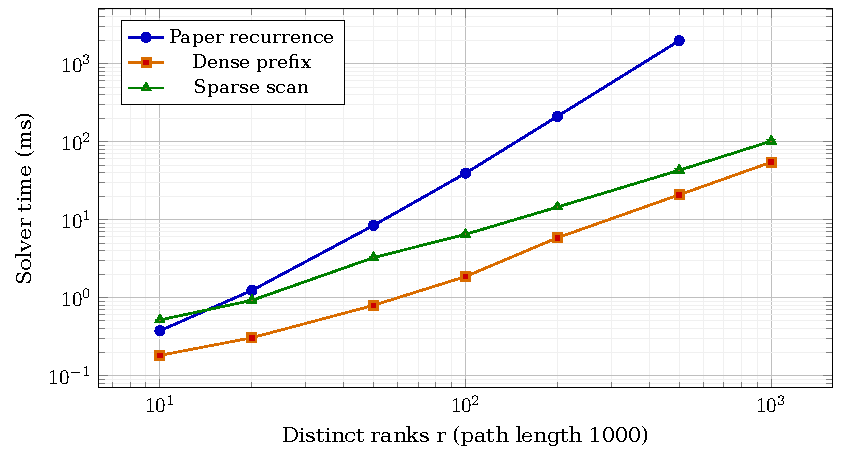
\includegraphics[width=0.94\linewidth]{../results/figures/forest-scaling.pdf}
\end{figure}

Trên TTSP dày, quét sự kiện đạt GM \TTSPGM{} lần so với ma trận truyền nội bộ. Với $k=256$, $r=32$, dữ liệu có $1\,024$ cạnh nền và $32\,768$ cạnh thời gian; trung vị giảm từ \TTSPMatrixTime{} ms xuống \TTSPEventsTime{} ms, tương đương \TTSPExampleSpeed{} lần. Đỉnh RSS lớn nhất qua bảy mẫu giảm từ \TTSPMatrixRSS{} xuống \TTSPEventsRSS{} MiB; đáp án dài $424$ bit. Đây là cải thiện cả thời gian và bộ nhớ trên cùng một bài toán, không phải kết quả tính theo mô-đun.

Một trường hợp bổ sung $k=32,r=128$ đạt tỷ số \TTSPExtraSpeed{} lần, nhưng không được dùng thay cho GM của họ TTSP dày. Trên trường hợp thưa có $r=\TTSPSparseRanks$, thuật toán sự kiện hoàn thành trong \TTSPSparseTime{} ms, còn ma trận bị bỏ qua theo giới hạn ngân sách. Vì không có số đo ma trận, báo cáo không suy ra tỷ số tăng tốc cho trường hợp này.

Trên cactus, quét tuyến khối đạt GM \CactusGM{} lần so với DP tổng quát; so sánh phản ánh lợi ích của thuật toán chuyên biệt khi nhận diện đúng cấu trúc. Trên partial 2-tree, DP tối giản đạt GM \PartialGM{} lần so với DP nội bộ cũ. Chỉ hàng rừng ở Bảng~\ref{tab:speedups} đối chiếu với truy hồi của bài báo gốc; các hàng khác không phải phép đo trực tiếp mã nguồn hoặc thời gian do tác giả bài báo công bố.

\section{Đóng góp của tối ưu và trường hợp khó}

Thực nghiệm loại bỏ từng tối ưu ở Bảng~\ref{tab:ablation} giúp giải thích nguồn cải thiện của DP. Xóa nhãn đầu cuối làm giảm số trạng thái tạo; bỏ đồng thời cắt tỉa và xóa nhãn đưa số trạng thái trở lại gần bản cũ. Giữ mọi bảng con làm tăng số trạng thái đồng thời sống nhưng không làm tăng số trạng thái phải tạo. Như vậy, giảm không gian trạng thái và giảm thời gian giữ bảng là hai tác động khác nhau, không nên đồng nhất với một chỉ số bộ nhớ duy nhất.

\begin{table}[htbp]{Đóng góp của từng tối ưu trên ba partial 2-tree ($n=24$, $r=8$).}
\label{tab:ablation}
\centering\small
\setlength{\tabcolsep}{4pt}
\renewcommand{\arraystretch}{1.16}
\begin{tabular}{p{6cm}rrr}
\toprule
Cấu hình & Thời gian (ms) & Trạng thái tạo & \shortstack{Trạng thái\\sống cực đại} \\
\midrule
DP nội bộ cũ & \num{32.4} & 18\,785 & 18\,785 \\
DP đầy đủ & \num{5.46} & 6\,801 & 854 \\
Không xóa nhãn đầu cuối & \num{11.8} & 11\,324 & 2\,197 \\
Không cắt tỉa và xóa nhãn & \num{24.9} & 18\,785 & 4\,957 \\
Không lọc cặp ghép & \num{6.49} & 6\,801 & 854 \\
Giữ mọi bảng con & \num{5.73} & 6\,801 & 6\,801 \\
\bottomrule
\end{tabular}
\par\vspace{3pt}\begin{minipage}{0.97\linewidth}\footnotesize Thời gian là trung bình nhân của ba trung vị; hai cột cuối là trung vị theo trường hợp. Số trạng thái sống là số trạng thái đồng thời đang được giữ, không phải số đỉnh đồ thị.\end{minipage}
\end{table}


Khi bỏ cắt tỉa, phép xóa nhãn đầu cuối cũng phải tắt vì điều kiện đúng của phép xóa phụ thuộc bậc được phép tại $s,z$. Hàng đó không đo riêng tác động của cắt tỉa. Thực nghiệm loại bỏ từng tối ưu chỉ dùng ba trường hợp; kết quả hỗ trợ cơ chế thuật toán, chưa đủ để khẳng định hiệu ứng giống nhau trên mọi phân bố đầu vào.

Đồ thị ladder kiểm tra miền rộng hơn cactus và truy vấn hai cực TTSP có sẵn. Với $c$ cột, truy vấn từ góc trên-trái đến góc dưới-phải có $2^{c-1}$ đường đi tĩnh. Bảng~\ref{tab:ladder} cho thấy thuật toán liệt kê bắt đầu hết giờ ở kích thước lớn, trong khi DP mới vẫn đếm chính xác ở $c=64$, nơi có $2^{63}$ tuyến tĩnh. Đây là bằng chứng cho khả năng tổng hợp nhiều nghiệm, không chỉ cải thiện hằng số trên số lượng đường đi nhỏ.

\begin{table}[htbp]{Ladder có độ rộng hai, $r=4$, đầu cuối trên-trái và dưới-phải.}
\label{tab:ladder}
\centering\small
\setlength{\tabcolsep}{4pt}
\renewcommand{\arraystretch}{1.16}
\begin{tabular}{lrrrr}
\toprule
Số cột $c$ & Đường đi tĩnh & Liệt kê (ms) & DP cũ (ms) & DP mới (ms) \\
\midrule
8 & $2^{7}$ & \num{0.25} & \num{3.73} & \num{0.876} \\
16 & $2^{15}$ & \num{138} & \num{9.07} & \num{2.04} \\
24 & $2^{23}$ & Hết giờ & \num{14.2} & \num{3.16} \\
64 & $2^{63}$ & Hết giờ & \num{40.6} & \num{9.38} \\
\bottomrule
\end{tabular}
\par\vspace{3pt}\begin{minipage}{0.97\linewidth}\footnotesize Mỗi số đo là trung vị của bảy mẫu. Hết giờ nghĩa là tiến trình không hoàn thành trong 3 giây; không thay bằng một thời gian giả để tính tỷ số tăng tốc.\end{minipage}
\end{table}


Các hạn chế còn lại gồm dữ liệu chủ yếu là dữ liệu sinh, số hạt giống ở một số phép đo ít và tần số CPU chưa cố định. Khi $w$ hoặc $r$ tăng, số trạng thái của DP vẫn có thể lớn. Do đó, kết quả hiện tại hỗ trợ đóng góp về thuật toán có cấu trúc và thực nghiệm tái lập, nhưng chưa xác lập ưu thế trên mọi mạng thực tế hoặc tính mới toàn diện so với toàn bộ văn liệu hiện hành.

\chapter{Kết quả đạt được và hướng phát triển}

\section{Kết quả và kiến thức thu được}

Đề tài đã xây dựng được một khung đếm chính xác dựa trên cấu trúc đồ thị. Đóng góp lý thuyết chính là cục bộ hóa điều kiện thời gian, giữ quan hệ liên thông qua biên và xóa nhãn không cần thiết ở hai đầu cuối. Khung này cho thuật toán đa thức khi treewidth cố định, với cận $\bigO(N(r+1)^6)$ trên partial 2-tree và hai đầu cuối tùy ý. Đây là phần khác biệt quan trọng so với việc chỉ tối ưu truy hồi trên rừng hoặc chỉ xử lý truy vấn trùng hai cực TTSP.

Về thuật toán chuyên biệt, tổng tiền tố giảm một bậc phụ thuộc số nhãn trên rừng; quét sự kiện tránh ma trận truyền dày trên TTSP và mở rộng sang cactus theo truy vấn. Về thực nghiệm, các đối chiếu không có sai lệch và phép đo lặp cho thấy tăng tốc trên các họ đã khảo sát, đồng thời làm rõ trường hợp hết giờ, giới hạn bộ nhớ và tác động riêng của các tối ưu.

Những kiến thức và kỹ năng gắn với công việc gồm mô hình hóa đối tượng đếm, xây dựng bất biến, tách điều kiện thời gian khỏi liên thông, phân tích số nguyên lớn và thiết kế thực nghiệm có đối chứng. Trọng tâm là giải thích tính đúng và hiệu quả trong miền áp dụng.

\section{Hướng nghiên cứu tiếp theo}

Ưu tiên tiếp theo là thẩm định độc lập chứng minh, đặc biệt ở bước ghép hai rừng và gộp nhãn đầu cuối, rồi đối chiếu có hệ thống với các công trình mới. Các kết quả trong báo cáo là đóng góp được đề xuất và kiểm chứng trong phạm vi đề tài; chưa thể thay thế quy trình phản biện khoa học bằng một kết luận về tính mới toàn cầu.

Về thuật toán, có thể nghiên cứu giảm số cặp ghép, khai thác thêm cấu trúc của partial 2-tree và tìm cận thấp hơn số mũ sáu theo $r$. Câu hỏi cụ thể là có thể giảm sự phụ thuộc nhãn tại biên mà vẫn bảo toàn tính đơn hay không; không giả định trước rằng phép định hướng sự kiện mở rộng được sang mọi đồ thị độ rộng hai.

Về thực nghiệm, cần thêm hạt giống, ổn định tần số CPU và bổ sung mạng thực tế. Hướng ứng dụng là tính chỉ số trung gian thời gian với định nghĩa đường đi tối ưu và phép giảm phù hợp. Các hướng này chưa được ghi nhận là kết quả hoàn thành.
\label{report:body:end}

\clearpage
\phantomsection
\addcontentsline{toc}{chapter}{Tài liệu tham khảo}
\begin{thebibliography}{9}
\begin{bibsection}{Tài liệu tiếng Anh}
\bibitem{enright2025}
Jessica Enright, Kitty Meeks và Hendrik Molter.
\textit{Counting Temporal Paths}. Algorithmica, 87, tr.~736--782, 2025.
\url{https://doi.org/10.1007/s00453-025-01301-3}.

\bibitem{eppstein1992}
David Eppstein. \textit{Parallel Recognition of Series-Parallel Graphs}.
Information and Computation, 98(1), tr.~41--55, 1992.
\url{https://doi.org/10.1016/0890-5401(92)90041-D}.

\bibitem{tarjan1972}
Robert Tarjan. \textit{Depth-First Search and Linear Graph Algorithms}.
SIAM Journal on Computing, 1(2), tr.~146--160, 1972.
\url{https://doi.org/10.1137/0201010}.

\bibitem{atlas}
NetworkX Developers. \textit{graph\_atlas\_g: Graph Atlas}.
Tài liệu chính thức; dữ liệu của đề tài lấy từ NetworkX 3.5.
\url{https://networkx.org/documentation/stable/reference/generated/networkx.generators.atlas.graph_atlas_g.html}.
Truy cập ngày 04/10/2026.
\end{bibsection}
\end{thebibliography}

\clearpage
% Leave comments, scores and signature to the evaluator.
\thispagestyle{empty}
\begingroup\setlength{\parindent}{0pt}
\begin{center}
  \includegraphics[height=2.7cm]{UET logo.pdf}\par
  \vspace{0.6cm}\textbf{Ý KIẾN ĐÁNH GIÁ}
\end{center}
\vspace{0.4cm}
\foreach \lineindex in {1,...,12}{\noindent\makebox[\linewidth]{\dotfill}\par\vspace{0.25cm}}
\vspace{0.65cm}\begin{center}
  Điểm số: \rule{1.6cm}{0.4pt}\qquad Điểm chữ: \rule{2cm}{0.4pt}
\end{center}
\vspace{0.7cm}\hfill\begin{minipage}{0.65\linewidth}\centering
  Hà Nội, ngày \rule{0.7cm}{0.4pt} tháng \rule{0.7cm}{0.4pt} năm \rule{1cm}{0.4pt}\par
  Giảng viên đánh giá\par\textit{(Ký, ghi rõ họ tên)}
\end{minipage}
\endgroup

\end{document}
